\documentclass[twoside]{article}
\setlength{\oddsidemargin}{0.25 in}
\setlength{\evensidemargin}{-0.25 in}
\setlength{\topmargin}{-0.6 in}
\setlength{\textwidth}{6.5 in}
\setlength{\textheight}{8.5 in}
\setlength{\headsep}{0.75 in}
\setlength{\parindent}{0 in}
\setlength{\parskip}{0.1 in}

\usepackage{graphicx}
\usepackage{url}
\graphicspath{ {Images/} }

%
% The following commands sets up the lecnum (lecture number)
% counter and make various numbering schemes work relative
% to the lecture number.
%
\newcounter{lecnum}
\renewcommand{\thepage}{\thelecnum-\arabic{page}}
\renewcommand{\thesection}{\thelecnum.\arabic{section}}
\renewcommand{\theequation}{\thelecnum.\arabic{equation}}
\renewcommand{\thefigure}{\thelecnum.\arabic{figure}}
\renewcommand{\thetable}{\thelecnum.\arabic{table}}
\newcommand{\dnl}{\mbox{}\par}

%
% The following macro is used to generate the header.
%
\newcommand{\lecture}[4]{
  \pagestyle{myheadings}
  \thispagestyle{plain}
  \newpage
  \setcounter{lecnum}{#1}
  \setcounter{page}{1}
  \noindent
  \begin{center}
  \framebox{
     \vbox{\vspace{2mm}
   \hbox to 6.28in { {\bf CMPSCI~590S~~~Systems for Data Science
                       \hfill Fall 2017} }
      \vspace{4mm}
      \hbox to 6.28in { {\Large \hfill Lecture #1  \hfill} }
%       \hbox to 6.28in { {\Large \hfill Lecture #1: #2  \hfill} }
      \vspace{2mm}
      \hbox to 6.28in { {\it Lecturer: #3 \hfill Scribe: #4} }
     \vspace{2mm}}
  }
  \end{center}
  \markboth{Lecture #1: #2}{Lecture #1: #2}
  \vspace*{4mm}
}

%
% Convention for citations is authors' initials followed by the year.
% For example, to cite a paper by Leighton and Maggs you would type
% \cite{LM89}, and to cite a paper by Strassen you would type \cite{S69}.
% (To avoid bibliography problems, for now we redefine the \cite command.)
%
\renewcommand{\cite}[1]{[#1]}

% \input{epsf}

%Use this command for a figure; it puts a figure in wherever you want it.
%usage: \fig{NUMBER}{FIGURE-SIZE}{CAPTION}{FILENAME}
\newcommand{\fig}[4]{
           \vspace{0.2 in}
           \setlength{\epsfxsize}{#2}
           \centerline{\epsfbox{#4}}
           \begin{center}
           Figure \thelecnum.#1:~#3
           \end{center}
   }

% Use these for theorems, lemmas, proofs, etc.
\newtheorem{theorem}{Theorem}[lecnum]
\newtheorem{lemma}[theorem]{Lemma}
\newtheorem{proposition}[theorem]{Proposition}
\newtheorem{claim}[theorem]{Claim}
\newtheorem{corollary}[theorem]{Corollary}
\newtheorem{definition}[theorem]{Definition}
\newenvironment{proof}{{\bf Proof:}}{\hfill\rule{2mm}{2mm}}

% Some useful equation alignment commands, borrowed from TeX
\makeatletter
\def\eqalign#1{\,\vcenter{\openup\jot\m@th
 \ialign{\strut\hfil$\displaystyle{##}$&$\displaystyle{{}##}$\hfil
     \crcr#1\crcr}}\,}
\def\eqalignno#1{\displ@y \tabskip\@centering
 \halign to\displaywidth{\hfil$\displaystyle{##}$\tabskip\z@skip
   &$\displaystyle{{}##}$\hfil\tabskip\@centering
   &\llap{$##$}\tabskip\z@skip\crcr
   #1\crcr}}
\def\leqalignno#1{\displ@y \tabskip\@centering
 \halign to\displaywidth{\hfil$\displaystyle{##}$\tabskip\z@skip
   &$\displaystyle{{}##}$\hfil\tabskip\@centering
   &\kern-\displaywidth\rlap{$##$}\tabskip\displaywidth\crcr
   #1\crcr}}
\makeatother

% **** IF YOU WANT TO DEFINE ADDITIONAL MACROS FOR YOURSELF, PUT THEM HERE:



% Some general latex examples and examples making use of the
% macros follow.

\begin{document}

%FILL IN THE RIGHT INFO.
%\lecture{**LECTURE-NUMBER**}{**DATE**}{**LECTURER**}{**SCRIBE**}
\lecture{5}{September 19}{Emery Berger}{Aishwarya Sudhakar, Kevin Feveck}

\section{Processes}

In UNIX land, to create a process we invoke \texttt{fork()} and the calling process is cloned. In the parent process, \texttt{fork()} returns the child's process ID (PID) while in the child process \texttt{fork()} returns 0. The child is a clone of the parent and resumes execution at the point after the call to \texttt{fork()}, however the child does not share any state with the parent. Each process has it's own memory space. 

For processes that are allocated a lot of memory, cloning can be expensive, especially as this memory copy must be done atomically to ensure that the values in memory do not change before they are copied to the child process state. This can take even longer if some memory in the parent process is paged out to disk. This idea of copying all of memory during the clone phase is called pre-emptive or eager copying. 

In actuality, this is not how \texttt{fork()} is implemented. It instead does what is called on-demand or lazy copying. Only what is needed is copied. Memory pointers, rather than actual values, are copied. When a parent or a child wants to modify a value in memory, a new page is allocated, the values copied to this new page, and then the modification is allowed to happen. This is called a copy-on-write, Copy-on-write ensures that the view of memory only changes for the process that writes/modifies, the other process will still point to the old value. 

\section{Processes vs Threads}
Since process creation implements a copy-on-write protocol, there is only a little more overhead when comparing process creation to thread creation. When should we use each? It depends. 

Threads communicate via shared memory. Processes do not share memory, and instead communicate via message passing (this is called Inter-Process Communication).

One downside to threads, is that if one thread goes down, due to a runtime error for example, the entire process running the threads is killed. This is not very good for designing fault-tolerant applications. With processes, if a process dies, it does not affect the other running processes. This 'dead' process, can simply be restarted (by a master process for example).

\section{Tolerating Errors}
Say a node has a failure rate of:\\

\centerline{$P_n (fail) = \frac{1}{100}$}

And node failures are independent of one another. If we add another node for redundancy purposes, the probability of failure of the system becomes:\\

\centerline{$P_s (fail) = P_n(fail) x P_n (fail) = \frac{1}{100} x \frac{1}{100} = \frac{1}{10000}$}

If we were to add a third redundant node (Trimodular redundancy), the failure rate of the system becomes:\\

\centerline{$P_s (fail) = \frac{1}{1000000}$}

In addition to redundancy, check-pointing can be implemented so that failed processes can be restarted from a previously known good "snapshot".

Random errors (due to cosmic rays for example) may corrupt bit values in memory. While there are mechanisms for dealing with this in memory (Parity bit, Error Correcting Code (ECC), Single Error Correct Double Error Detect (SECDED)) we can also take a majority vote among our redundant systems. It is unlikely that two will fail, especially in the same way, unless the error is deterministic.

There are two types of bugs that may error in a system: a Bohr bug (deterministic) and a Heisenbug (non-deterministic). Bohr bugs are good from the programmer perspective because they are reproducible and can be easier to debug. This is not the case with Heisenbugs; they are much harder for the programmer to reproduce and debug. From the user perspective, deterministic errors mean the system will always fail under these conditions, and this is a bad thing. Heisenbugs are much more tolerable, since the process/task can be restarted and will probably complete this time. 

\section{How to increase reliability}

The notion of reliability with independent systems is achieved through a backup. There are different kinds of backup:

\begin{description}
  \item[$\bullet$ Periodical Backup] At defined checkpoints, a snapshot of the system is stored in disk. The snapshot includes the state of the system from the last successful checkpoint. This is also called incremental backup
  \item[$\bullet$ Full Backup] At defined checkpoints, a snapshot of the entire system is taken and stored in disk.
\end{description}


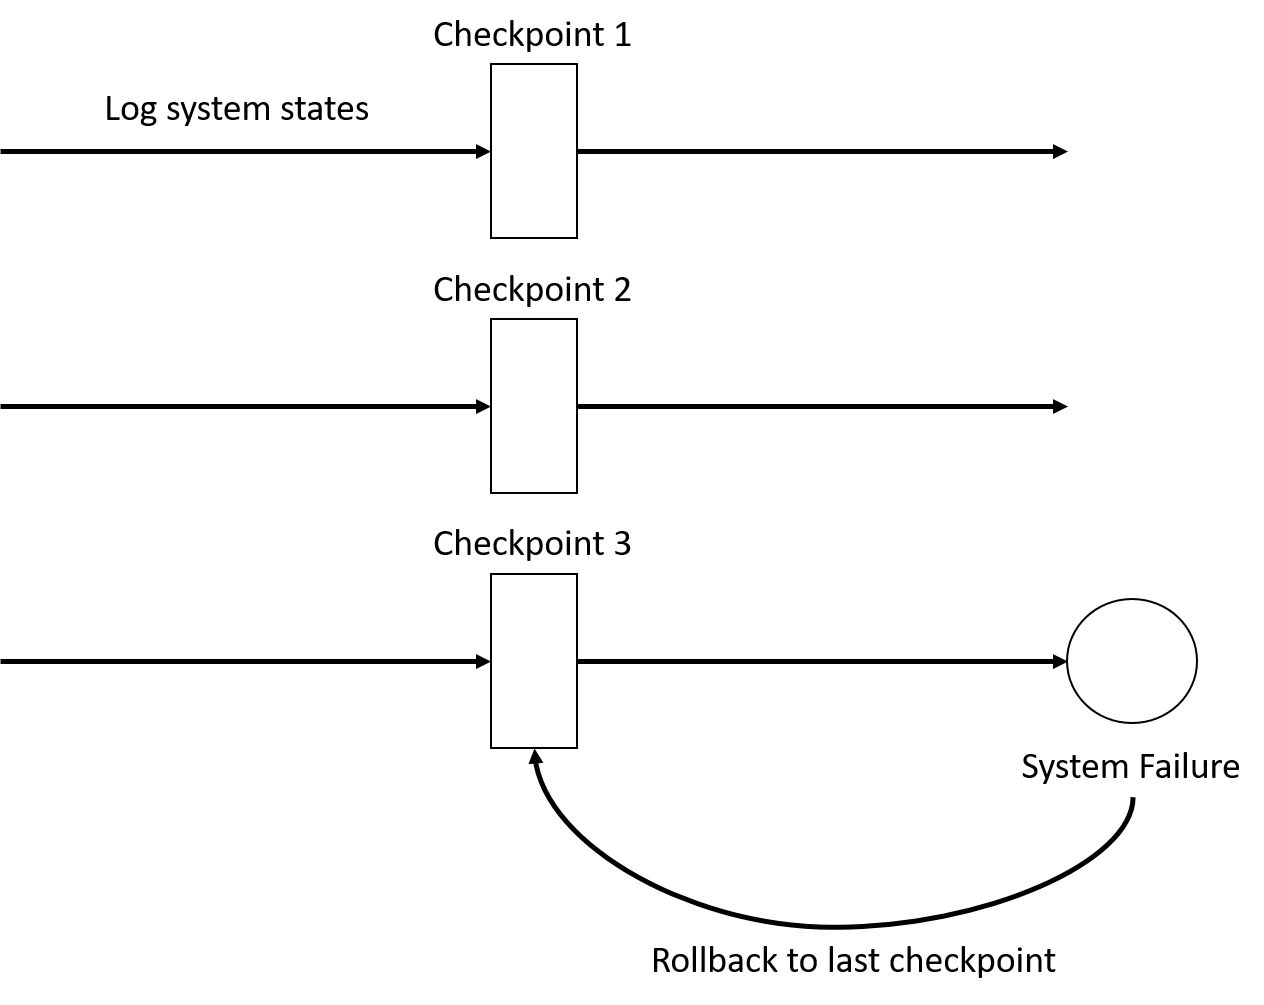
\includegraphics[scale=0.2]{Scribe-Drawings-Reliability.png}


When a failure is incurred, the system rolls back to the last checkpoint, restores its state from the backup and continues processing. There is no significant loss in data. The machines use logs to record the state of the system.

\section{Master-Slave Architecture}

One of the most common architecture of distributed systems is the Master-Slave architecture. This has now been rephrased to Master-Worker architecture. This design includes one of the systems which takes care of the other systems in the cluster. The master is fundamental in scheduling the tasks and also in verifying the health of a worker in the cluster. The master periodically pings the workers of their status, if the worker machines fail to respond, the master then notes these machines as dead and reschedules the tasks assigned to the dead machine to another machine in the cluster. 

\centerline{$P_m (fail) =  \frac{1}{100}$}
\centerline{$P_m (sucess) =  1 - \frac{1}{100} = \frac{99}{100}$}


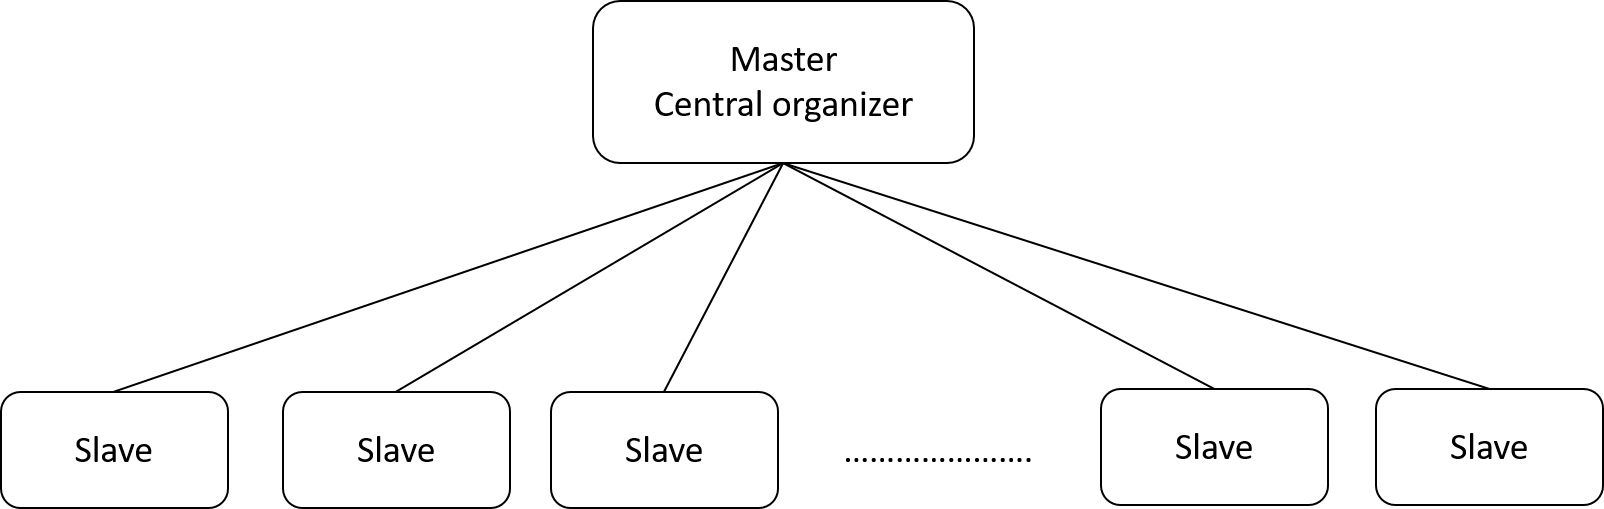
\includegraphics[scale=0.2]{Scribe-Drawings-MasterSlave.png}


The odds of a master failing are negligible. But in cases where the master fails, the other workers in the cluster hold a  \textbf{Leader-Election} process, where the workers contend amongst each other to decide who becomes the next master. 

\end{document}
